%!TEX root = ../../main.tex
\subsection{Hyperledger Fabric}
\label{ch:approach:intro:hyperledger}
Hyperledger Fabric is an open-source enterprise-grade permissioned \ac{DLT} platform designed for use in enterprise contexts that delivers crucial differentiating capabilities over other popular distributed ledger or blockchain platforms. It was established under the Linux Foundation and currently holds the solid support of enterprises and developers for continuous improvement. 
Important features:
\begin{itemize}
    \item Highly modular and configurable architecture, enabling innovation, versatility, and optimization for various industry use cases (banking, finance, insurance, healthcare, human resources, supply chain, digital music delivery, and others.).
    
    \item First distributed ledger platform to support chaincode\footnote{In Hyperledger Fabric Smart Contracts are bettern known as "chaincode"} authored in a general-purpose programming language (Java, Go, and Node.js), facilitating their development without learning a new language or \ac{DSL}.
    
    \item Permissioned platform. Unlike public permissionless networks, the participants are known to each other. While the participants may not fully trust one another (they may be competitors in the same industry), a network can be operated under a governance model built off what trust exists between participants, such as a legal agreement or framework for handling disputes.

    \item Support for pluggable consensus protocols enables the platform to be more effectively customized to fit particular use cases and trust models. By default, Fabric implements BFT consensus fully but could be modified instead for another  \ac{CFT} consensus protocol when fewer parties or organizations participate.

    \item Can leverage consensus protocols that do not require a native cryptocurrency to incent costly mining or fuel smart contract execution. Avoidance of a cryptocurrency reduces some significant risk/attack vectors, and the absence of cryptographic mining operations means that the platform can be deployed with roughly the exact operational cost as any other distributed system.

    \item Enables privacy and confidentiality of transactions and chaincode.

\end{itemize}
 
These differentiators make Fabric one of the better performing platforms available today regarding transaction processing and confirmation latency. 

\subsubsection{Hyperledger Fabric Components}

\begin{figure}[!h]
    \centering
    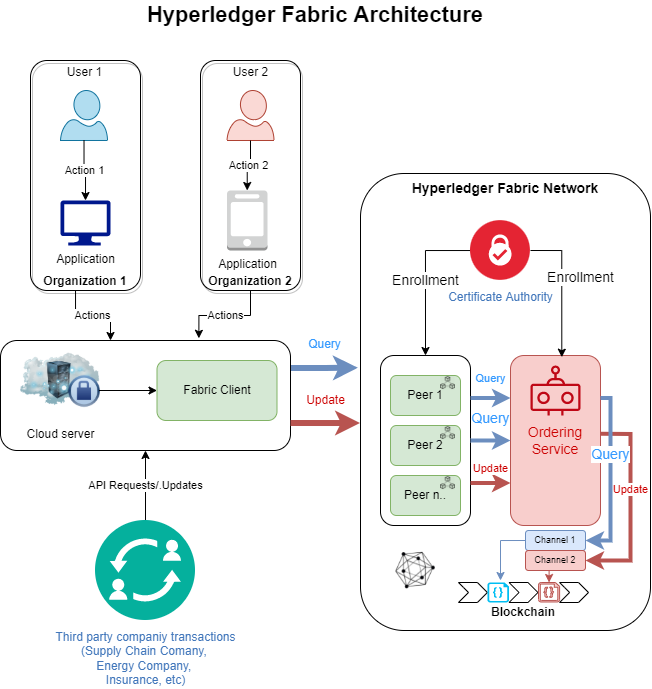
\includegraphics[width=15cm]{img/Hyperledger_Architecture.png}
    \caption{Hyperledger Fabric Architecture}
    \label{fig:HyperledgerArchitecture}
\end{figure}

\begin{itemize}
\item \textbf{Organization}. Virtual representation of a company/organization. Can define the areas and users that the organization will allow to interact with the \ac{DLT} 
\item \textbf{User}. Defines the entity that will directly interact with the ledger via \emph{Fabric Client} through a \ac{PKI} provided by a \ac{CA}.
\item \textbf{Application}. Is a custom software used by the organization and able to communicate with the ledger. The application will communicate with the ledger by sending actions to the \emph{Fabric Client}.
\item \textbf{Cloud server}. Infrastructure that hosts and provides the \emph{Fabric Client} that can directly communicate with the ledger.
\item \textbf{Fabric Client}. Application built by Hyperledger or custom code able to send query or update instructions to the ledger by invoking chaincode functions.
\item \textbf{Third-party companies}. Other organizations with custom applications or network infrastructure can also communicate with \emph{Fabric client} whenever the \ac{CA} grants access to the ledger.
\item \textbf{Certificate Authority}. Authorization service provider which uses \ac{PKI}-based certificates to network member organizations and their users. Issues one root certificate to each member and one enrollment certificate to each authorized user.
\item \textbf{Peer}. Servers that host a copy of the blockchain. Peers belong to the Organizations, and different organizations can have more than zero peers. The peers are coordinated by the ordering service and some of them will be selected as endorsers to validate chaincode transactions.
\item \textbf{Ordering Service} is in charge of ordering the transactions. An orderer or set of orderer nodes form an ordering service. Because Fabric’s design relies on deterministic consensus algorithms, any block validated by the peer is guaranteed to be final and correct. This architecture promotes finality by separating the endorsement of chaincode execution (which happens at the peers) from ordering, which provides advantages in performance and scalability as it eliminates bottlenecks.
\item \textbf{Channel}. Is a private tunnel (subnet) of communication between one or more organizations through which the parties agree over one or more chaincode instructions. Whenever organizations join a party, no other external entity is able to see the interactions between then, ensuring external anonymity and inner transparency. Peers can join one or more channels. Each channel has its own chain of blocks.
\item \textbf{Blockchain}. Is the ledger of the infrastructure, it exists in the peers and communicates via a single channel.
\end{itemize}

\subsubsection{Hyperledger Fabric Workflow}
The following steps form part of a typical Fabric workflow configuration:
\begin{enumerate}
    \item A user invokes a chaincode execution through his application, which generates a transaction invocation. Client broadcasts the transaction invocation request to the Endorser peer
    \item The Endorser peer checks the Certificate to validate the transaction. If verification is approved,it simulates the transaction by generating a response with a read-write set. Afterwards endorses the generated response using its own certificate. If the transaction fails a rejection response is sent.
    \item The client receives the endorsed proposal responses from Endorsing Peers.
    \item The client now sends the approved transaction to the orderer peer for this to be properly ordered and be included in a block.
    \item The orderer node includes the transaction into a block.
    \item The orderer node broadcasts the generated block to all Peers (to both Endorsing Peers and Committing Peers) on the relevant channel. Then, each Peer ensures that each transaction in the received block was signed by the appropriate Endorsing Peers. These individual peers then update their local ledger with the latest block. Thus all the network gets the ledger synced.
    \item The Clients receive any subscribed events if any.
    
\end{enumerate}

\begin{figure}[!h]
    \centering
    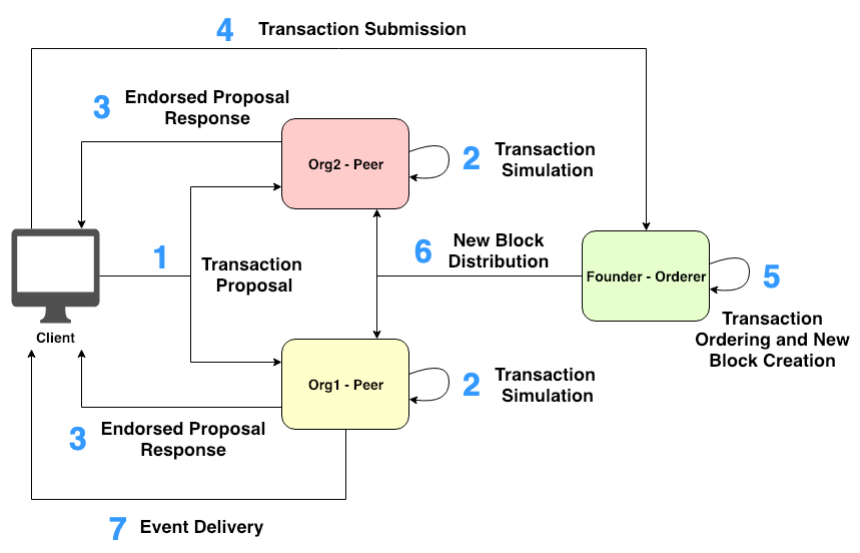
\includegraphics[width=15cm]{img/HyperledgerWorkflow.png}
    \caption{Hyperledger Fabric General Workflow}
    \label{fig:HyperledgerWorkflow}
\end{figure}